
%\section{Calibration and Validation}
\section{Validation}
\label{sec:validation}

% VALIDATION TODO
%
% show major effort
% table of results
% show hierarchy
% precisely define cases 
%
%

%
% meshed vanes are 24x more expensive
%

The previous sections briefly outlined the physical phenomenon under
consideration, the mathematical models proposed to simulate it,
and the numerical solution of these models for a variety of system 
configurations and scenarios. Before these simulations can be used 
as a tool to evaluate proposed system designs,
it is necessary to validate that the model accurately represents reality.  
This section contains a discussion of the validation of the computational models
against existing experimental data and high fidelity simulations.

A challenge in this project is the scarcity of experimental data. Only two or three cases of 
experimental measurements are available. These measurements, for reasons detailed in the next subsection, 
are not sufficient to provide confidence in the output of simulations across a wide variety 
of scenarios. Thus, a high fidelity model using explicitly gridded vanes with enforced no-slip 
velocity boundary conditions on the surface of the vane has been developed. These ``gridded'' runs have been
evaluated against the experimental data, where they match quite closely. However, as 
detailed in \ref{subsec:vane}, explicitly meshing the vanes would be far too prohibitively expensive to 
permit a rapid exploration of a variety of system configurations. Instead, this high fidelity model is used 
as a means to generate additional truth data to permit validation of lower fidelity models, such as the virtual vanes. 
Likewise, the results of the unsteady virtual vane simulations can be used as validation data for a further 
reduced order, steady navier-stokes model. This hierarchy of validation is depicted in \ref{fig:val_hier}, with 
data sources that generate more reliable data at the top, and models that are less reliable, but also 
less computationally expensive at the bottom. In terms of expense, the reduced order model (ROM) 
generates a solution in approximately two minutes, versus twelve hours for the unsteady virtual vane model. 
The gridded vanes require another factor of ten in computational time, and many more man-hours hours of work
to generate the mesh. Therefore, it is unrealistic to perform parameter sweeps or system configuration investigations
with the gridded vanes. Instead, the ROM is used, with promising results re-evaluated in the unsteady VV models, 
and so on up the hierarchy if more confidence is necessary. 
The remainder of this section discusses the validations performed between
the different models and the experimental data. 

 \begin{figure}[!htb]
   \begin{center}
    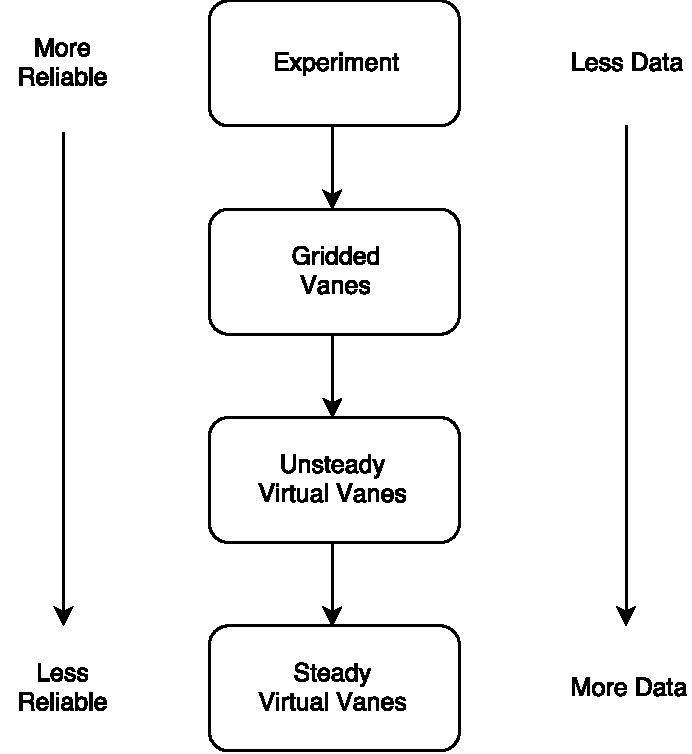
\includegraphics[width = 12 cm]{figs/validation_hierarchy}
    \caption{This figures depicts the validation hierarchy between different 
      sources of data generation. The experimental measurements lies at the top, 
      where the data is expected to be the most reliable, but simultaneously the most rare. 
      Moving down the table leads to simulated data sources that are less reliable but 
      increasingly cheaper in time to generate. At the bottom is the reduced order model (ROM).}
    \label{fig:val_hier}
   \end{center}
 \end{figure}

%
%
%
%
% http://www.tablesgenerator.com/
%

%
% experimental challenges
%

\subsection{Experimental Data}

Experimental data has been generated 
The existing available data from the ``truth'' cases (experiment and gridded vanes) 
are summarized in table \ref{tab:val_data}. 

\large
\begin{table}[h]
\centering
\label{my-label}
\begin{tabular}{l|l|l|}
           & Wind                      & Thermal-Only              \\
  \hline 
Experiment & Straight Vanes $60^{\circ}$ & Straight Vanes $60^{\circ}$ \\
           &                           & Straight Vanes $30^{\circ}$ \\
           &                           & Hybrid                    \\
  \hline 
Gridded    & Straight Vanes $60^{\circ}$ & Straight Vanes $60^{\circ}$ \\
           & Straight Vanes $30^{\circ}$ & Straight Vanes $30^{\circ}$ \\
  \hline 
\end{tabular}
  \caption{Presently available data from experiment and 
    the gridded vanes. }
  \label{tab:val_data}
\end{table}

The general system configuration is depicted in Figure \ref{fig:lab_image}. 
Several challenges arise in performing a validation comparison between the
simulation output and the experimental data. These data were taken using
particle image velocimetery (PIV), and the errors in 
in measurement and sampling are not known. 
In addition, only velocity measurements are available. Several
potentially important quantities of interest, such as the pressure field
or the temperature, have not been measured.\todo{need to describe the experiment}


%  \begin{figure}[!htb]
%    \begin{center}
%     \includegraphics[width = 12 cm]{figs/lab_setup}
%     \caption{The single tier straight vane laboratory configuration. The
%     apparatus is shown with a turbine, but it was removed for data
%     gathering.}
%     \label{fig:lab_image}
%    \end{center}
%  \end{figure}

While no sensitivity analysis has been performed, it is likely that the
largest uncertainty in the laboratory simulation is a result of the
ventilation. The heated plate at the bottom of the apparatus
generates enough heat to cause a significant increase in room
temperature (30+ Kelvin), which greatly impacts the SoV
performance, as the ground to air thermal gradient drives the
vortex. The laboratory is cooled to maintain
temperature, in particular, two inlet HVAC ducts into the room. 
%While efforts have been made to characterize the level of ventilation being
%used, these numbers come with non-trivial uncertainties attached. 
One vent runs continuously at 288 Kelvin with a flow rate estimated 
to be 1 $m^3$/s.
%(4-6 m/s with an approximate area of 0.2 $m^2$)
The other vent is active only if the room temperature exceeds 301 Kelvin, 
with a flow rate also estimated at 1 $m^3$/s.
Finally, the air leaves through the cracks around the laboratory doors and 
exhaust vents. 
Preliminary results indicated that an
inflow rate of 1 $m^3$/s, the lower bound of the possible inflow rates 
results in excessive heating of the room, while inflow conditions at the 
maximum inflow rate of 2 $m^3$/s result in a simulated room that 
is too cold, compared to the laboratory. 

Our simulated vortices are sensitive to ambient room temperature and thus 
the inflow rate. It is likely that the laboratory is run where one of
the vents is operating intermittently. 
To mimic these conditions in our simulations, Dirichlet boundary conditions 
on parts of the sides of the computational domain are used to
establish a constant inflow of cool air at the rates 
proscribed by our collaborators. Over the remainder of the side walls, 
adiabatic thermal boundary conditions are are used. 

The most signficant boundary condition disparity is that
flow leaves the domain through the top boundary, instead of out
of the sides of the room. Preliminary results suggested that the SoV phenomenon 
was not sensistive to these boundary condition details. The important element is the 
global energy balance in the room. The flow rate into the room is adjusted to 
1.3 $m^3$/s for the validation results discussed here. 


  \begin{figure}[!htb]
    \begin{center}
     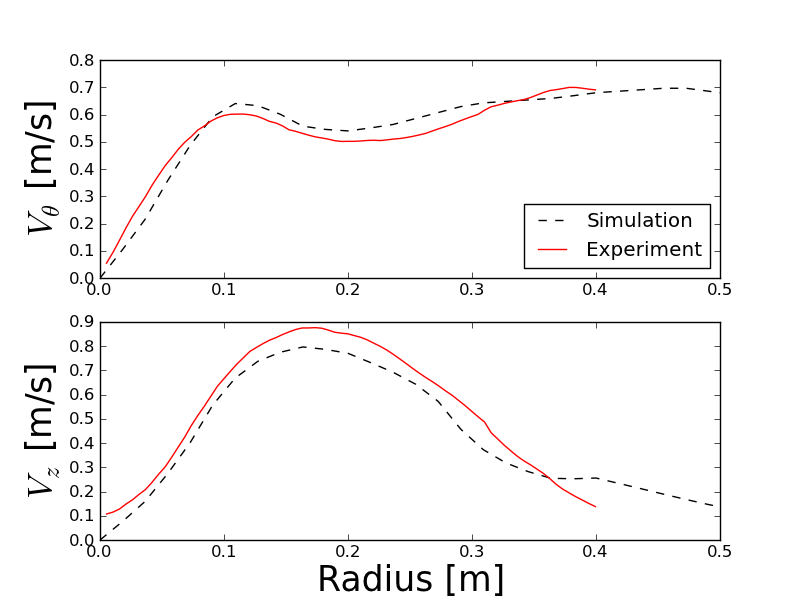
\includegraphics[width = 12 cm]{figs/hybrid_profile}
     \caption{Azimuthal and vertical velocity profiles as a function of
     radius. The simulation and experimental data broadly agree, with
     the simulation also exhibiting the characteristic ``twin-peak''
     structure of the hybrid vanes in the azimuthal velocity. }
     \label{fig:lab}
    \end{center}
  \end{figure}

Figure \ref{fig:lab} is a direct comparisons between laboratory measurements for a simple 
two tier configuration ($55^{\circ}$ top, $30^{\circ}$ bottom)\todo{add gridded vanes} and 
a nominally identical simulation. The simulation and experiment broadly
agree. The simulation correctly reproduces the twin peak structure in
the azimuthal velocity observed for this configuration in the
experiment. The radial location of peak vertical velocity also closely
agrees with experiment. The largest observed difference is near the
center, where the simulation predicts a downward vertical velocity, in
contrast to the modest vertical flows measured in the laboratory.  

Similar validation comparisons have been made between several other
configurations, notably the $30^{\circ}$ and $60^{\circ}$ singly tier
straight vane cases, with similar levels of agreement. This represents
the totality of quantitiative data available for comparison. Qualitative
comparisons have been made between the our simulation results with a
mean velocity and with wind tunnel pictures. These images showed roughly
consistent structure between simulation and
experiment. Finally. estimates of the energy fluxes between the field
configuration and our simulation results agreed within 15\%. These
validation studies have provided a modest level of confidence that our
simulations accurately reproduce the dynamics observed in real vane
configurations.\todo{incomplete, should reflect entire validation plan} 

%
% validation story is incomplete
% 
% you have done: 
%
% 1) comparions between laboratory + gridded + virtual 
% 
% 2) comparisons between gridded + virtual in laboratory
%    + field configurations, thermal only and wind
%
% 3) comparisons of virtual vanes to field observations 
%    quantitative + qualitative
%
%
% You need to discuss what needs to be validated -- the
% comparison to gridded vanes is a useful validation tool 
%
